\section{Evaluación tiempo de activación usando APIs}
El tipo de prueba que se realizó se basa en el trabajo realizado por \cite{tesis-monsalve-rodrigo} y \cite{tesis-meneses-sebastian}. En ambos trabajos se considera el tiempo de las tres etapas comprendidas por: el tiempo de la generación de mensajes, el tiempo de envío y el tiempo de activación de actuatores en el Software Arduino. En este proyecto, se considera el tiempo de generación de mensajes en la API de alto nivel (C\# y Java), el tiempo que demora en llegar al Servidor WebSocket, el tiempo de la generación de mensajes desde la instancia de OpenGlove en el servidor, luego el tiempo hasta software de control en la placa Arduino, el tiempo a través del Bluetooth, para finalmente calcular el tiempo que demora el microcontrolador Arduino en realizar la activación de los actuatores. Se realizaron 2000 pruebas entre la activación y desactivación, utilizando un Baudrate de 57600 y un LoopDelay igual a 0 ms en la placa Arduino. 
Los tiempos entre activación y desactivación desde la API de alto nivel, están dados por la velocidad entre cada mensaje que llega desde el software de control, evitando así, los efectos indeseados por el envío de mensajes en corto tiempo.

Se realizaron pruebas desde uno a cinco motores físicos disponibles en la placa. El dispositivo utilizado para la evaluación técnica de las APIs fue el Samsung Galaxy S5 Mini. La Figura \ref{fig:csharp-api-test} muestra la aplicación desarrollada con Xamarin.Forms para realización de las evaluaciones técnicas de la API C\#  y la Figura \ref{fig:java-api-test}, muestra la aplicación desarrollada para la realización de evaluaciones técnicas de la API Java.

\begin{figure}
 \begin{center}
   	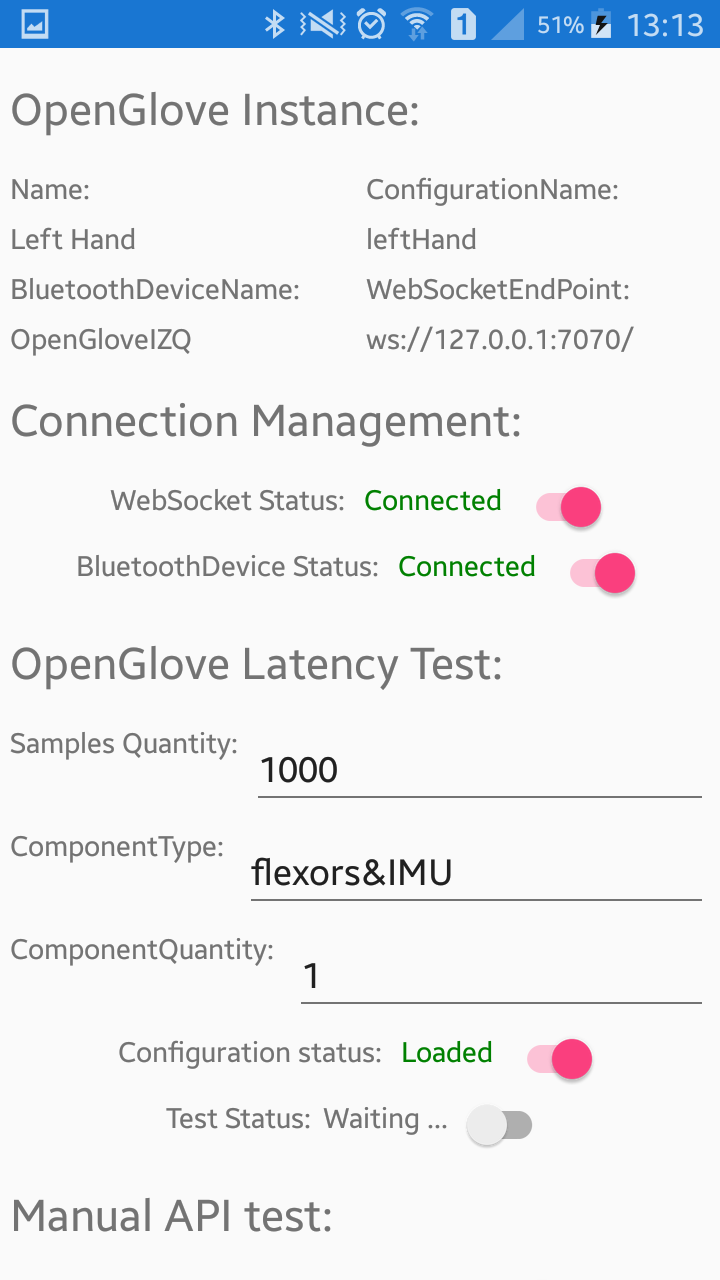
\includegraphics[width=0.3\textwidth]{images/chapter05/C-Sharp-APITest.png}
   \centering
   \captionsetup{justification=centering}
    \caption[Aplicación utilizada para realizar las pruebas de la API C\# ]{Aplicación utilizada para realizar las pruebas de la API C\# \\Fuente: elaboración propia (2018)} 
    \label{fig:csharp-api-test}
  \end{center}
\end{figure}

\begin{figure}
 \begin{center} 
   	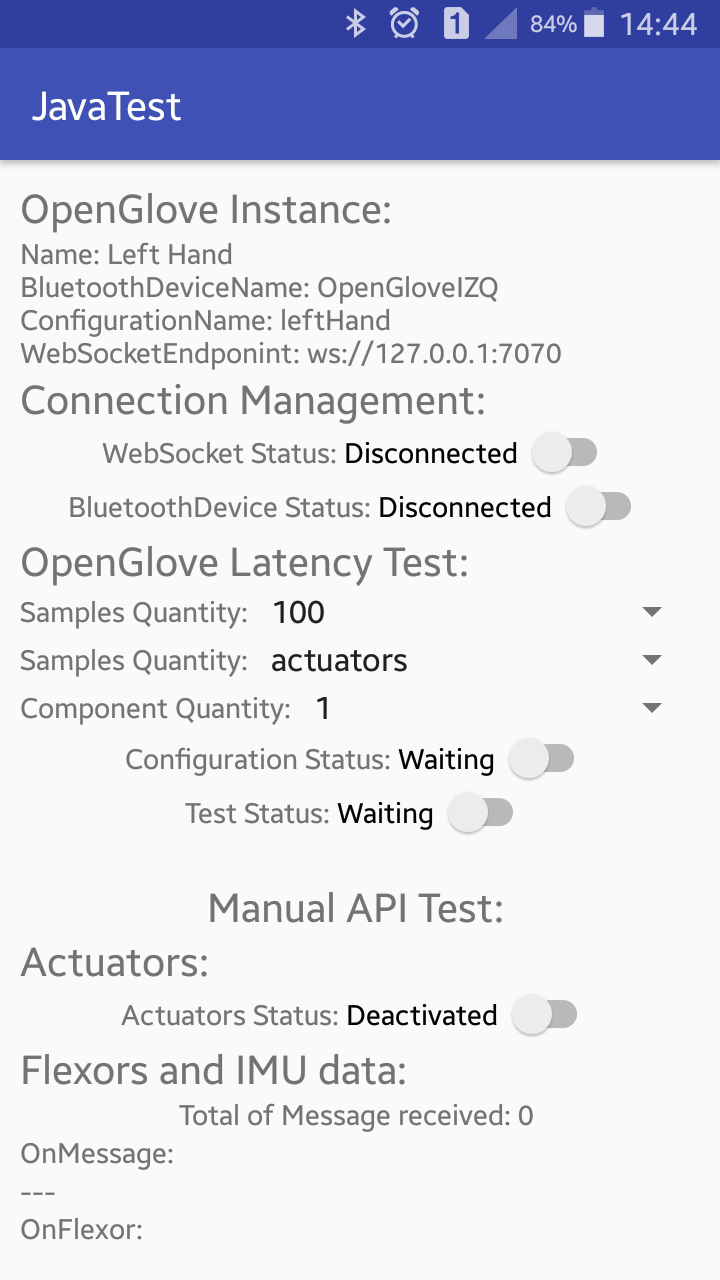
\includegraphics[width=0.3\textwidth]{images/chapter05/Java-APITest.png}
   \centering
   \captionsetup{justification=centering}
    \caption[Aplicación utilizada para realizar las pruebas de la API Java ]{Aplicación utilizada para realizar las pruebas de la API Java \\Fuente: elaboración propia (2018)} 
    \label{fig:java-api-test}
  \end{center}
\end{figure}
 
 % Baudrate Arduino Control  Software = 57600 bits per second
\subsection{API C\#}
Para realizar las evaluaciones técnicas de esta API, fue necesario desarrollar una aplicación en Xamarin.Forms mostrada en la Figura \ref{fig:csharp-api-test}, que hiciera uso de la API y registrara los tiempos de latencia obtenidos en el dispositivo Android.

% {START} RESUME TABLE ---------------------------------
%\caption[Resumen resultado pruebas de activación usando API C\#]{Resumen resultado pruebas de activación usando API C\# en $\mu s$\\ Fuente: Elaboración propia (2018)}
%\label{table:motor-xamarin-galaxy-api}

% & $\mu s$ & $\mu s$ & $\mu s$ & $\mu s$ & $\mu s$ &     & \\ 

% Table created by stargazer v.5.2.2 by Marek Hlavac, Harvard University. E-mail: hlavac at fas.harvard.edu
% Date and time: Tue, Sep 04, 2018 - 15:40:15
\begin{table}[!htbp] \centering 
\captionsetup{justification=centering}
\caption[Resumen resultados de los tiempos de activación usando API C\#]{Resumen resultados de los tiempos de activación usando API C\# en $\mu s$\\ Fuente: Elaboración propia (2018)}
\label{table:motor-xamarin-galaxy-api}
\begin{tabular}{@{\extracolsep{5pt}} cccccccc} 
\\[-1.8ex]\hline 
\hline \\[-1.8ex] 
motors & Mean & Median & Min & Max & Std. Dev. & Skewness & Kurtosis \\ 
            & $\mu s$ & $\mu s$ & $\mu s$ & $\mu s$ & $\mu s$ &     & \\ 
\hline \\[-1.8ex] 
$1$ & $9,447.961$ & $9,519.400$ & $3,478.700$ & $22,064.100$ & $4,011.735$ & $0.625$ & $2.841$ \\ 
$2$ & $10,505.070$ & $10,292.400$ & $4,241.800$ & $23,386.200$ & $4,083.306$ & $0.615$ & $2.712$ \\ 
$3$ & $10,573.240$ & $9,208.100$ & $5,214.200$ & $23,436.100$ & $3,868.327$ & $0.683$ & $2.598$ \\ 
$4$ & $12,915.820$ & $13,147.200$ & $5,894.100$ & $25,246.200$ & $4,018.170$ & $0.383$ & $2.716$ \\ 
$5$ & $13,497.350$ & $13,429$ & $6,513.400$ & $25,496$ & $3,900.305$ & $0.410$ & $2.665$ \\ 
\hline \\[-1.8ex] 
\end{tabular} 
\end{table} 
% {END} RESUME TABLE ---------------------------------

La Figura \ref{fig:xamarin-galaxy-hist-motors}, muestra los histogramas de las latencias obtenidas al mandar los mensajes de activación y desactivación. Se realizaron pruebas desde uno a cinco motores.

\begin{figure}
 \begin{center} 
   	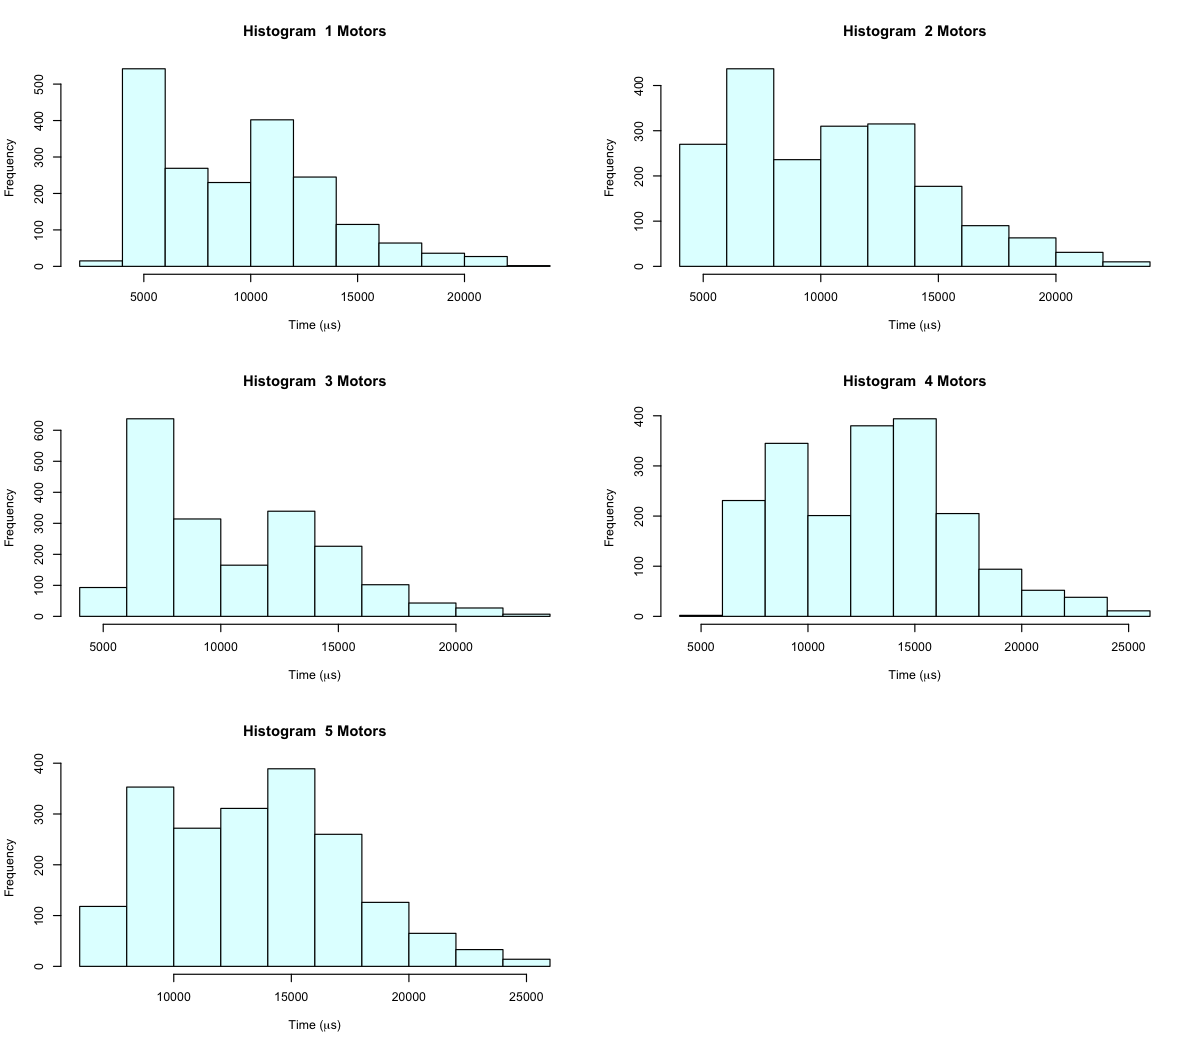
\includegraphics[width=1.0\textwidth]{evaluation/graphics/Xamarin/Galaxy-APITest/HistMotorsXamarinGalaxy-APITest.png}
   \centering
   \captionsetup{justification=centering}
    \caption[Histogramas de los tiempos de activación de motores usando API C\# ]{Histogramas de los tiempos de activación de motores usando API C\# \\Fuente: elaboración propia (2018)} 
    \label{fig:xamarin-galaxy-hist-motors-api}
  \end{center}
\end{figure}

\begin{figure}[H]
  \begin{center} 
   	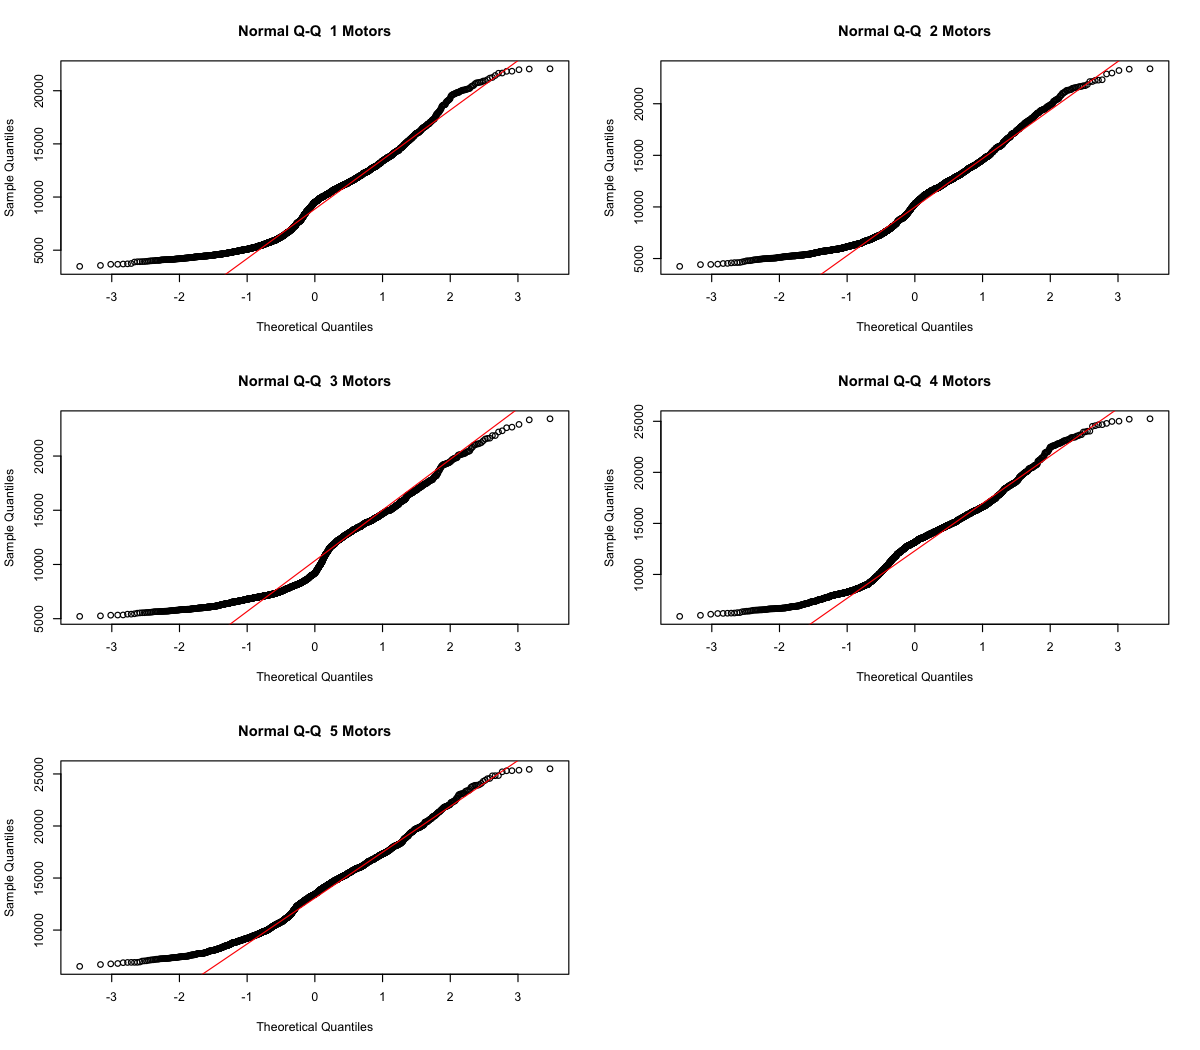
\includegraphics[width=1.0\textwidth]{evaluation/graphics/Xamarin/Galaxy-APITest/NormalQQMotorsXamarinGalaxy-APITest.png} 
   	\centering
   	\captionsetup{justification=centering}
    \caption[Gráfico QQ delos tiempos de activación de motores usando API C\# ]{Gráficos QQ de los tiempos de activación de motores usando API C\# \\Fuente: elaboración propia (2018)} 
    \label{fig:xamarin-galaxy-QQ-motors-api}
  \end{center}
\end{figure}

\begin{figure}[H]
  \begin{center} 
   	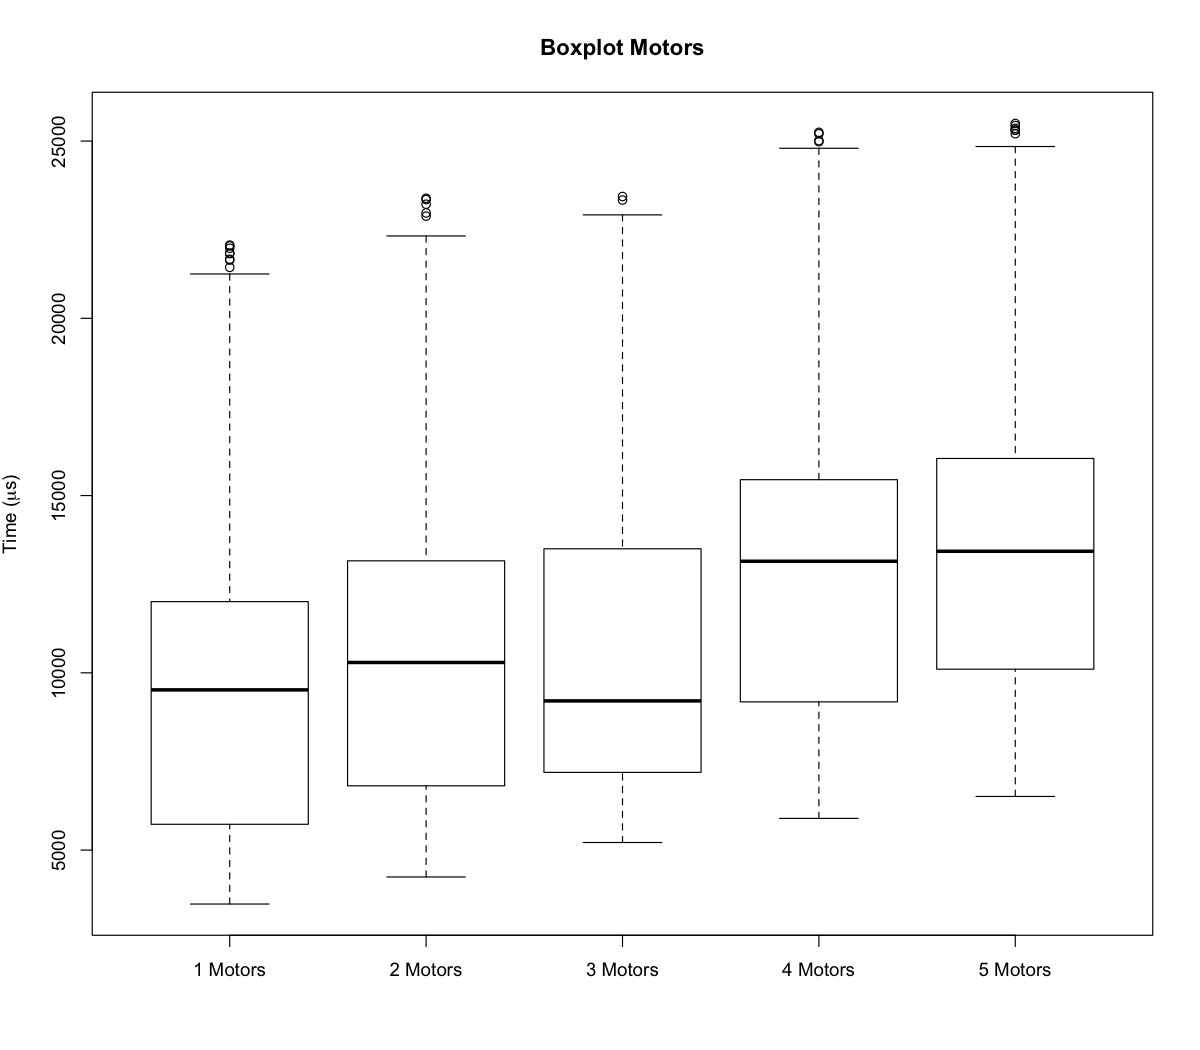
\includegraphics[width=0.8\textwidth]{evaluation/graphics/Xamarin/Galaxy-APITest/BoxplotMotorsXamarinGalaxy-APITest.png} 
   	\centering
   	\captionsetup{justification=centering}
    \caption[Gráficos de cajas de los tiempos de activación de motores usando API C\# ]{Gráficos de cajas de los tiempos de activación de motores usando API C\# \\Fuente: elaboración propia (2018)} 
    \label{fig:xamarin-galaxy-boxplot-motors-api}
  \end{center}
\end{figure}




\subsection{API Java}
Para realizar las evaluaciones técnicas de esta API, fue necesario desarrollar una aplicación nativa en Android mostrada en la Figura \ref{fig:java-api-test}, que hiciera uso de la misma para registrar las latencias obtenidas en las pruebas.
